\chapter{Alterações nos Nomes das Telas}
\label{detalhes:transicao-e-ajustes}

\section{Tabela De-Para}


\begin{table}[!h]
	\begin{center}
		\begin{tabular}{|c|c|}
			\hline
			\rowcolor{corCOULD!80} \multicolumn{2}{|c|}{\Large Nomes das Funcionalidades \normalsize} \\ \hline
			\rowcolor{corCOULD!80} \multicolumn{2}{|c|}{\Large Tabela ``De-Para'' de Alterações \normalsize} \\ 
			\rowcolor{corCOULD!80} \multicolumn{2}{|c|}{\large (Telas da Barra Lateral do Sistema) \normalsize} \\ \hline

			% CABEÇALHO        
			\rowcolor{lightgray}\textbf{De} & \textbf{Para} \\ \hline
			% CONTEÚDO
			% Código escrito manualmente
			\rowcolor{cldfC1!40} \cellcolor{corCOULD!10} Gerenciar Perfil & Administrar Perfis  \\ \hline
			\rowcolor{cldfC1!40} \cellcolor{corCOULD!10} Gerenciar Usuário & Administrar Usuários  \\ \hline
			\rowcolor{cldfC1!40} \cellcolor{corCOULD!10} Gerenciar Unidade & Administrar Unidades  \\ \hline

			\rowcolor{cldfC1!40} \cellcolor{corCOULD!10} Gerenciar e Analisar Ordem de Serviço & Gerenciar e Analisar Solicitações  \\ \hline



		\end{tabular}    
		\caption{\label{tab:gerosassel:analise1} De Para de Alterações nos Nomes}
	\end{center}
\end{table}

%\toGil{Confirmar com Gilberto} Confirmado na reuniao do dia 19/09/2022

\textbf{As alterações devem ocorrer:}

\begin{itemize}
	\item Na barra lateral do sistema:
	
	\centering
	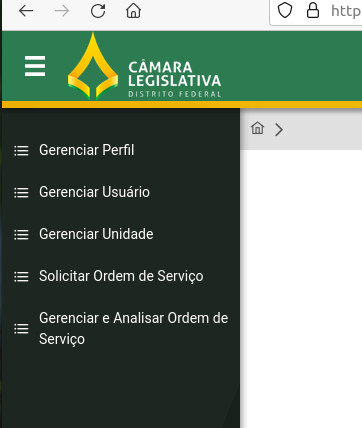
\includegraphics[width=0.8\textwidth]{fig/detalhes/barra-lateral.png}
	
	
	\item No texto das ``funcionalidades'' da tela ``Gerenciar Perfis'':

	\centering
	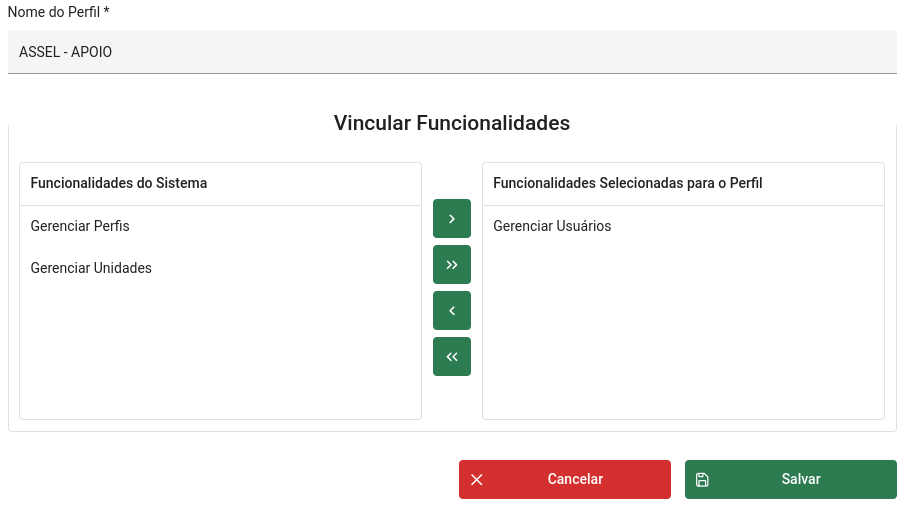
\includegraphics[width=0.8\textwidth]{fig/detalhes/vincular-funcionalidades.png}
\end{itemize}

